\section{Mediciones}

Para tomar las mediciones, creamos grupos de subconjuntos de jugadores con nombres arbitrarios, variando la cantidad de subconjuntos, el tamaño máximo de los subconjuntos y el número total de jugadores.

Además, notamos que los procesos de fondo del sistema nos generaba distorciones en los tiempos de ejecución de una misma muestra. Resolvimos este problema realizando varias mediciones para el mismo escenario de subconjuntos y tomando el promedio de los tiempos obtenidos. Esta estrategia nos permitió abordar otro problema significativo: el orden en el que se evalúan los jugadores en cada subconjunto adquiere una importancia relevante en el rendimiento final del algoritmo. Esto depende especialmente de la frecuencia con la que cada jugador aparece en los demás subconjuntos. 

Asimismo, al definir arbitrariamente cada escenario, puede ocurrir que en una cantidad 
$m$ de subconjuntos, los jugadores incluidos en cada uno sean considerablemente diferentes o poco comunes, lo que representa un caso desfavorable. En contraste, en una cantidad de conjuntos $m+1$, podría darse una situación mucho más favorable, con una mayor similitud entre los jugadores incluidos en cada conjunto. Esto puede llevar a una diferencia significativa en los tiempos de ejecución, a pesar de que la cantidad de conjuntos varíe en una sola unidad.

Tanto en mediciones temporales como en mediciones de aproximación, comparamos el efecto de modificar una variable por vez, tanto $m$ como $b$. Estas mediciones se realizaron sobre los diferentes algorítmos analizados a lo largo del informe: Backtracking, algorítmo Greedy Máximo por Grupo, algorítmo Greedy Máximo Global con Recálculo, Programación Lineal Entera y Programación Lineal Continua.

Al evaluar el algoritmo de Backtracking, podemos corroborar a través de los gráficos una clara tendencia exponencial en el tiempo de ejecución conforme se incrementa la cantidad de subconjuntos (figs. \ref{fig:medicion_t_backtracking_var_m}). Sin embargo, al observar el gráfico de la figura \ref{fig:medicion_t_backtracking_var_b}, se puede apreciar que el tiempo de ejecución disminuye a medida que se incrementa el tamaño máximo de los subconjuntos. Esto se debe a que nuestra implementación de backtracking hace grandes podas cuando se repiten muchos jugadores entre conjuntos. Un mayor tamaño de los conjuntos implica un aumento en la probabilidad de intersecciones grandes entre los mismos.

\begin{figure}[h]
    \centering
    \begin{minipage}{0.45\textwidth}
        \centering
        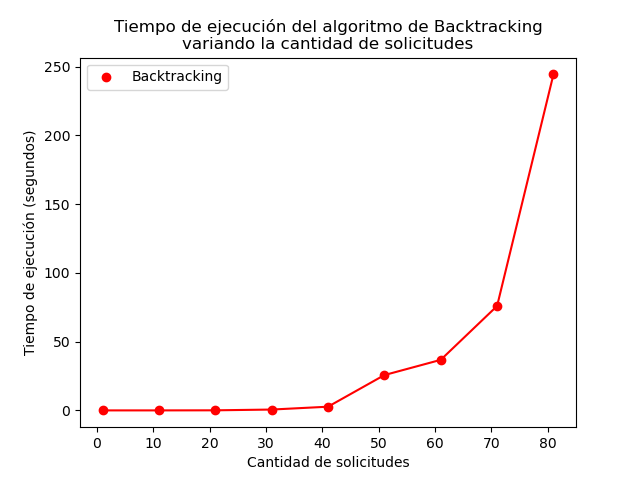
\includegraphics[width=\textwidth]{img/medicion_t_backtracking_var_m.png}
        \caption{Backtracking: Medición de tiempos variando $m$.}
        \label{fig:medicion_t_backtracking_var_m}
    \end{minipage}\hfill
    \begin{minipage}{0.45\textwidth}
        \centering
        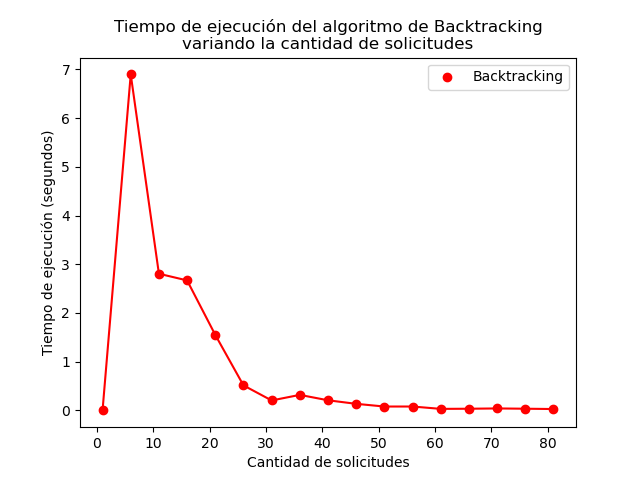
\includegraphics[width=\textwidth]{img/medicion_t_backtracking_var_b.png}
        \caption{Backtracking: Medición de tiempos variando $b$.}
        \label{fig:medicion_t_backtracking_var_b}
    \end{minipage}
\end{figure}

Por otro lado, el algoritmo de Programación Lineal Entera, contrario a lo esperado, presenta una gráfica más cercana a una función lineal (figs. \ref{fig:medicion_t_pl_var_m} y \ref{fig:medicion_t_pl_var_b}), asemejandose en tiempo de ejecución con el algorítmo de Programación Lineal Continua. Esto se debe a las optimizaciones implementadas en la librería \texttt{pulp}, las cuales reducen significativamente su tiempo de ejecución en comparación con su complejidad teórica. Es importante mencionar que la visualización de una curva exponencial en este algoritmo solo ocurre en situaciones donde las optimizaciones no influyen de manera considerable.

\begin{figure}[h]
    \centering
    \begin{minipage}{0.45\textwidth}
        \centering
        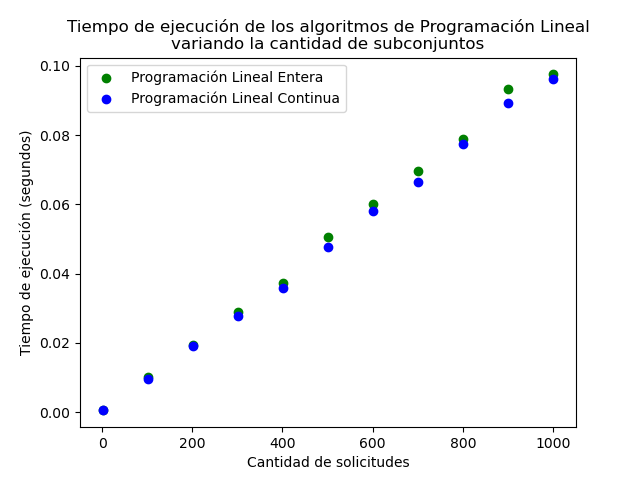
\includegraphics[width=\textwidth]{img/medicion_t_pl_var_m.png}
        \caption{Programación Lineal: Medición de tiempos variando $m$.}
        \label{fig:medicion_t_pl_var_m}
    \end{minipage}\hfill
    \begin{minipage}{0.45\textwidth}
        \centering
        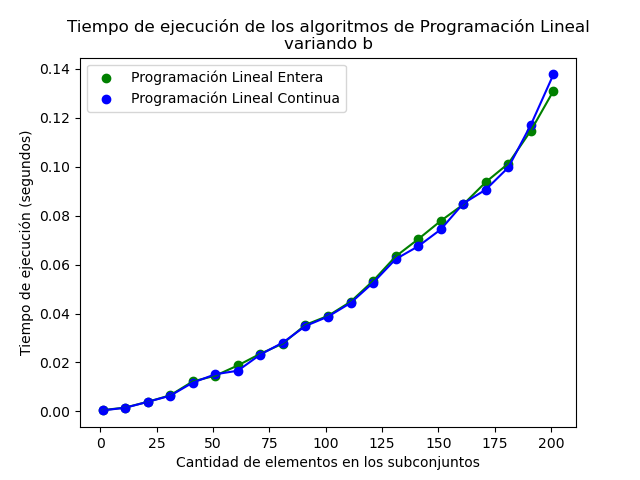
\includegraphics[width=\textwidth]{img/medicion_t_pl_var_b.png}
        \caption{Programación Lineal: Medición de tiempos variando $b$.}
        \label{fig:medicion_t_pl_var_b}
    \end{minipage}
\end{figure}

En el siguiente gráfico, se ilustra el grado de aproximación, variando $m$, manteniendo $b=25$, (fig. \ref{fig:medicion_r_pl_var_m}) y variando $b$, manteniendo $m$ constante (fig. \ref{fig:medicion_r_pl_var_b}). La peor aproximación en la figura de la izquierda es $\approx 1.9\leq b-1$. En la figura de la derecha se puede observar que $r$ está muy lejos de superar $b-1$.

\begin{figure}[h]
    \centering
    \begin{minipage}{0.45\textwidth}
        \centering
        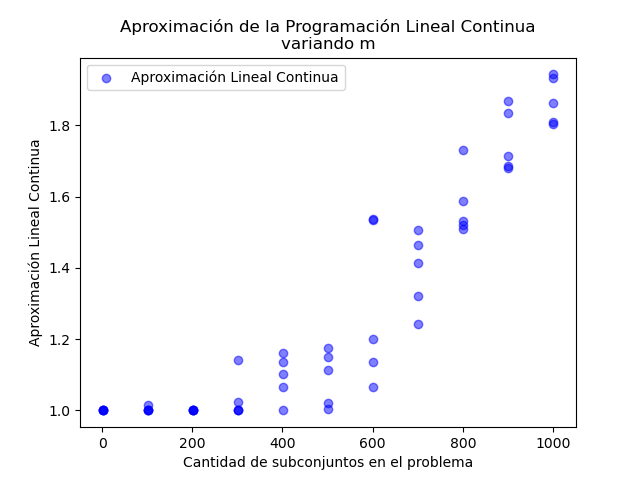
\includegraphics[width=\textwidth]{img/medicion_r_pl_var_m.png}
        \caption{Greedy: Relación entre $r(A)$ y $m$ para $b$ constante.}
        \label{fig:medicion_r_pl_var_m}
    \end{minipage}\hfill
    \begin{minipage}{0.45\textwidth}
        \centering
        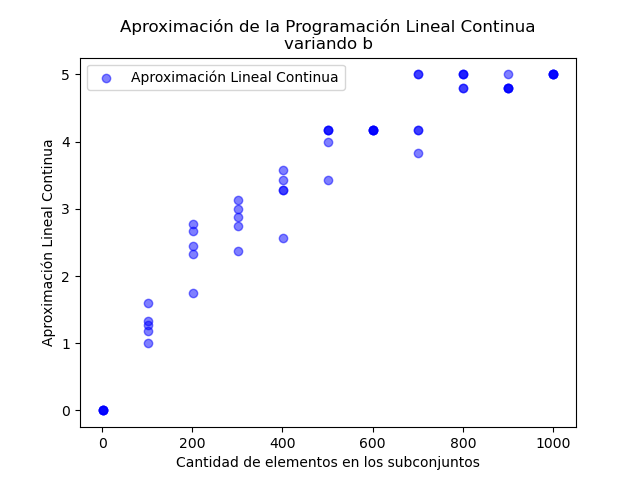
\includegraphics[width=\textwidth]{img/medicion_r_pl_var_b.png}
        \caption{Greedy: Relación entre $r(A)$ y $b$ para $m$ constante.}
        \label{fig:medicion_r_pl_var_b}
    \end{minipage}
\end{figure}

Por otra parte, al examinar los algoritmos que emplean la estrategia de diseño Greedy, se evidencia en la figura \ref{fig:medicion_t_greedy_var_m} que Máximos por Grupos tiene una tendencia lineal respecto a $m$, mientras que Máximo Global con Recálculo, una tendencia polinomial. En la figura \ref{fig:medicion_t_greedy_var_b} podemos ver que la complejidad de ambos algoritmos tiende a ser lineal para mayores valores de $b$ como consecuencia del mismo fenomeno observado en Backtracking donde se generan mayores intersecciones entre los grupos. Asimismo, se destaca una marcada diferencia en los tiempos de ejecución entre los dos algoritmos Greedy. A pesar de que el primero es más rápido, en las figuras \ref{fig:medicion_r_greedy_var_m} y \ref{fig:medicion_r_greedy_var_b_1} se expone que el segundo se acerca más a la solución óptima en todos los casos estudiados.

\begin{figure}[h]
    \centering
    \begin{minipage}{0.45\textwidth}
        \centering
        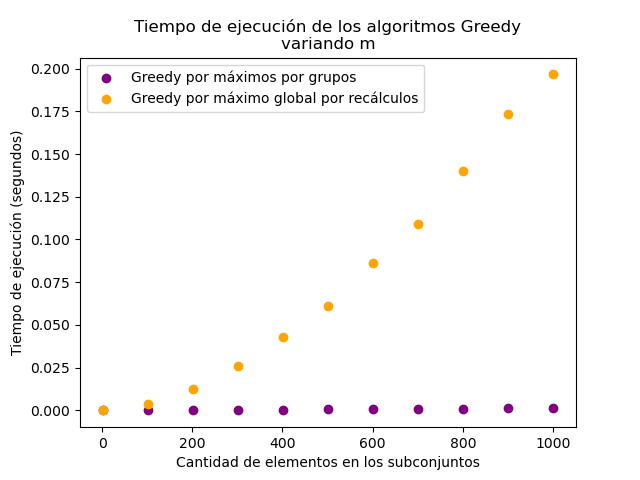
\includegraphics[width=\textwidth]{img/medicion_t_greedy_var_m.png}
        \caption{Greedy: Medición de tiempos variando $m$.}
        \label{fig:medicion_t_greedy_var_m}
    \end{minipage}\hfill
    \begin{minipage}{0.45\textwidth}
        \centering
        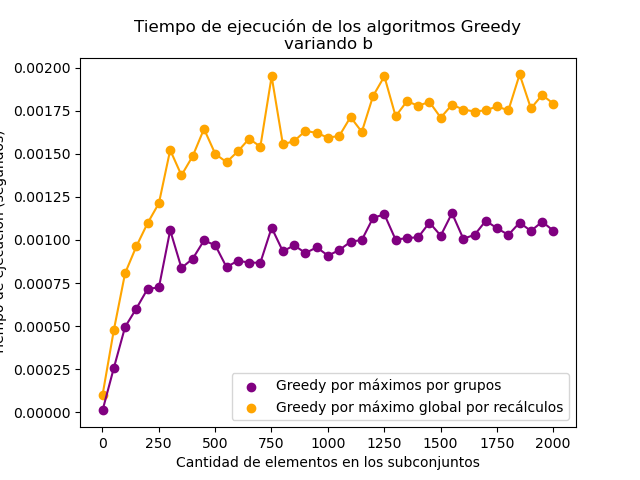
\includegraphics[width=\textwidth]{img/medicion_t_greedy_var_b.png}
        \caption{Greedy: Medición de tiempos variando $b$.}
        \label{fig:medicion_t_greedy_var_b}
    \end{minipage}
\end{figure}

Es interesante observar como el factor de aproximación $r(A)=\frac{A(I)}{z(I)}$ varía respecto a $m$ y a $b$. Para valores $b$ pequeños constantes, que es donde los dos algorítmos Greedy tienden a performar peor, se aprecia una tendencia polinomial respecto a la variación de $m$ (fig. \ref{fig:medicion_r_greedy_var_m}). Sin embargo, con $m$ constante, se puede observar una tendencia inversamente proporcional entre $r(A)$ y $b$ (fig. \ref{fig:medicion_r_greedy_var_b_2}). Esto se debe a que, con grupos más grandes, la probabilidad de que un elemento pertenezca a más de un grupo es mayor, llegando al punto de que exista uno o varios jugadores en la intersección de todos los conjuntos. Ambos algoritmos greedy obtienen siempre la solución óptima en este caso, por lo que $\lim\limits_{b \rightarrow \infty}r(A)=1$.

\begin{figure}[h]
    \centering
    \begin{minipage}{0.45\textwidth}
        \centering
        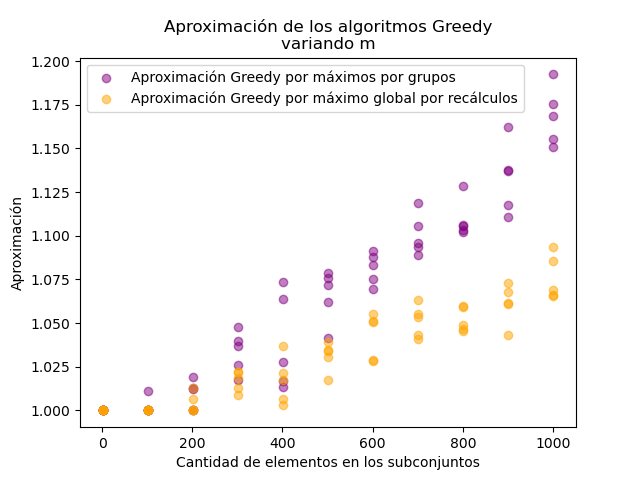
\includegraphics[width=\textwidth]{img/medicion_r_greedy_var_m.png}
        \caption{Greedy: Relación entre $r(A)$ y $m$ para $b$ constante.}
        \label{fig:medicion_r_greedy_var_m}
    \end{minipage}\hfill
    \begin{minipage}{0.45\textwidth}
        \centering
        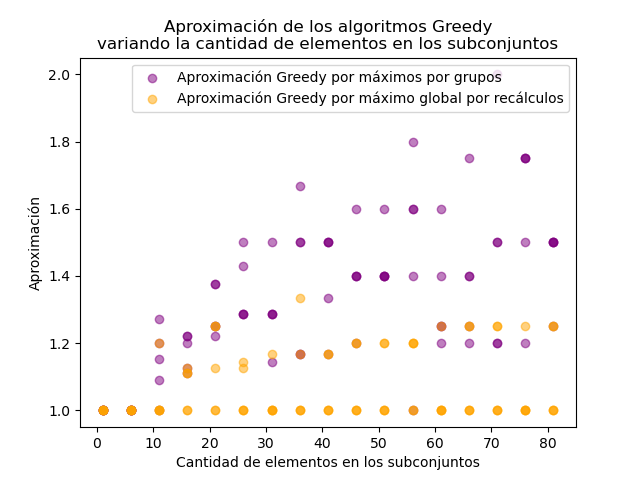
\includegraphics[width=\textwidth]{img/medicion_r_greedy_var_b_1.png}
        \caption{Greedy: Relación entre $r(A)$ y $b \in [0,100]$ para $m$ constante.}
        \label{fig:medicion_r_greedy_var_b_1}
    \end{minipage}\hfill
    \begin{minipage}{0.45\textwidth}
        \centering
        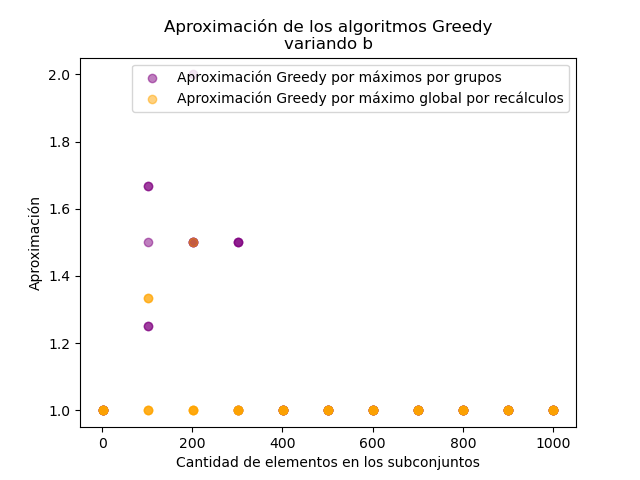
\includegraphics[width=\textwidth]{img/medicion_r_greedy_var_b_2.png}
        \caption{Greedy: Relación entre $r(A)$ y $b \in [0,1000]$ para $m$ constante.}
        \label{fig:medicion_r_greedy_var_b_2}
    \end{minipage}
\end{figure}

La decisiónn de qué algoritmo Greedy es el más adecuado cambia respecto a la sotiaco+pm. Por un lado, el algoritmo por grupo se destaca por su eficiencia temporal, ofreciendo tiempos de ejecución notoriamente inferiores y, por otro lado, el enfoque global muestra una mayor aproximación a la solución óptima.

Además realizamos mediciones con volumenes de datos inmanejables para los algoritmos de solución exacta, con el fin de corroborar de forma empírica la cota del algoritmo de Programacion Lineal Continua. Para ello implementamos un algoritmo que genera un set de conjuntos con una solución óptima menor o igual a un número $k$ (en nuestros ejemplos $k=25$). De esta manera, podemos corroborar dicha cota, conociendo la máxima solución óptima (decimos que es menor o igual porque pueden haber casos donde la generación aleatoria de subconjuntos implique elementos repetidos, lo que radica en una solución con un cardinal menor al impuesto por $k$).

En los dos primeros casos, se generaron combinando 2 y 3 letras por elemento, mientras que en el tercero se usaron solamente 2 letras. Esta variedad se buscó con el fin de ampliar las minimizar las colisiones (pero mantener suficientes como para que no sean todos los jugadores diferentes). En todos los casos, el tamaño de los subconjuntos oscila entre $10$ y $12$ elementos como mínimo y máximo, respectivamente.


Lo que podemos observar es que en estos casos generados (buscados meticulosamente) nuestro algoritmo de Greedy por Máximo Global con Recálculo tiene la solución óptima de las 3, con un tiempo de ejecución mediano, mientras el peor desempeño lo tiene el algoritmo de Programación Lineal Continua, con un tiempo de ejecución muy alto, y una solución muy lejana a la óptima, y el algoritmo de Greedy por Máximo por Grupo, con el tiempo de ejecución más bajo de todos, pero con una solución no siempre óptima.


En estos los casos generados, nuestro algoritmo de Greedy por Máximo Global con Recálculo ha logrado obtener la solución con cardinal más pequeño entre las tres, aunque este algoritmo alcanza un tiempo de ejecución promedio. 
Por otro lado, el desempeño más deficiente lo muestra el algoritmo de Programación Lineal Continua, con un tiempo de ejecución muy alto y soluciones distantes de la óptima. En contraste, el algoritmo de Greedy por Máximo por Grupo destaca por su tiempo de ejecución más reducido, aunque su solución no siempre alcanza la óptima.

Además la cota teórica calculada para Programacion Lineal Continua se cumple en todos los casos. 


\textbf{5000 subconjuntos, con 2 letras, 10 mínimo b, 12 máximo b, $|C|\leq 25$} 

\begin{itemize}
    \item Programación Lineal Continua:

    Cantidad mínima: 36

    Tiempo de ejecución: 336.2557799999997 milisegundos
    
    \item Greedy por Máximo Global con Recálculo:
    
    Cantidad mínima: 14
    
    Tiempo de ejecución: 13.29740200000007 milisegundos
    
    \item Greedy Máximo por Grupos:
    
    Cantidad mínima: 16
    
    Tiempo de ejecución: 6.6933350000000225 milisegundos
\end{itemize}

\textbf{5000 subconjuntos, con 3 letras, 10 mínimo b, 12 máximo b, $|C|\leq 25$}

\begin{itemize}
    \item Programación Lineal Continua:

    Cantidad mínima: 36

    Tiempo de ejecución: 336.2557799999997 milisegundos


    \item Greedy por Máximo Global con Recálculo:

    Cantidad mínima: 14

    Tiempo de ejecución: 13.29740200000007 milisegundos


    \item Greedy Máximo por Grupos:

    Cantidad mínima: 16

    Tiempo de ejecución: 6.6933350000000225 milisegundos

\end{itemize}

\textbf{10000 subconjuntos, con 2 letras, 10 mínimo b, 12 máximo b, $|C|\leq 25$}

\begin{itemize}

    \item    Programación Lineal Continua:
    
    Cantidad mínima: 35

    Tiempo de ejecución: 1460.1356119999998 milisegundos


    \item Greedy por Máximo Global con Recálculo:
    
    Cantidad mínima: 8

    Tiempo de ejecución: 50.457938999999726 milisegundos


    \item Greedy Máximo por Grupos:
    
    Cantidad mínima: 10

    Tiempo de ejecución: 30.84798200000005 milisegundos

\end{itemize}